\chapter{Grundlagen}
\section{Test-Driven Development}
Bei dem Test-Driven Development (TDD), zu Deutsch auch „test-getriebene Entwicklung“, handelt es sich um ein Entwicklungs- und Designverfahren für Software, bei dem Testfälle bereits vor oder spätestens parallel zur Implementierung spezifiziert werden. Die zu erstellende Software wird quasi über Tests entworfen. \cite[S. 151]{schatten_best_2010}

TDD sollte bereits bei der Anforderungsanalyse angewendet werden. Die Anforderungen sind so zu definieren, dass sichergestellt werden kann, dass die Erfüllung dieser Anforderungen mithilfe von Tests validiert werden können. Dies kann durch Testdefinitionen in Textform gewährleistet werden, in die genau die Vorbedingungen, die Ausführung und die zu erwartenden Ergebnisse beschrieben werden. \cite[S.188] {kleuker_qualitatssicherung_2019}

Die Abbildung \ref{schematischer Ablauf TDD} zeigt exemplarisch einen schematischen Ablauf des Test-Driven Development-Ansatzes. Am Anfang wird der Testfall definiert (Test Definition, TD), darauf folgt die Umsetzung und Programmierung (Programming, P). Im Anschluss werden die Testfälle ausgeführt (Test Execution, TE). \cite[S. 151]{schatten_best_2010}

\begin{figure}[h]
	\centering
	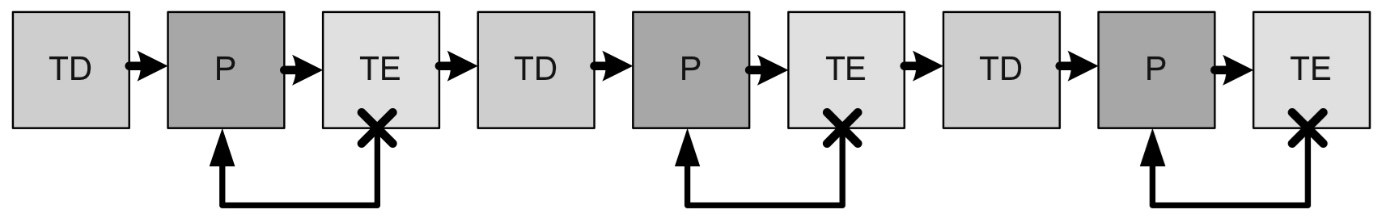
\includegraphics[clip,width=1\linewidth]{images/schematischer Ablauf TDD.jpg}
	\caption[schematischer Ablauf des Test-Driven Development]{schematischer Ablauf des Test-Driven Development \cite[S. 151]{schatten_best_2010}}
	\label{schematischer Ablauf TDD}
\end{figure}

Im Gegensatz dazu wird beim traditionellen Testen erst parallel zur Entwicklung oder nach Abschluss der Implementierung geeignete Testfälle definiert und ausgeführt, wie ein schematischer Ablauf in Abbildung \ref{schematischer Ablauf traditionelles Testen} zeigt. \cite[S. 150]{schatten_best_2010}

\begin{figure}[h]
	\centering
	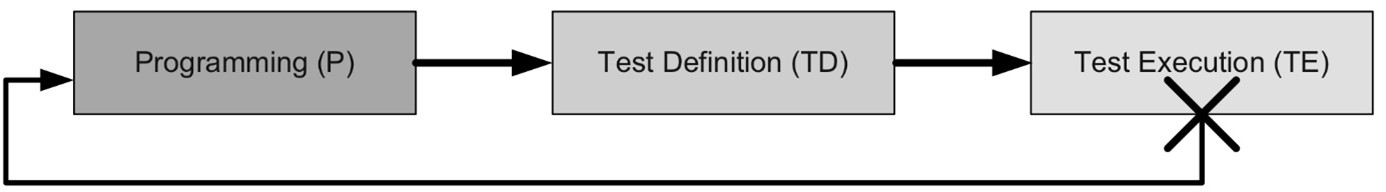
\includegraphics[clip,width=1\linewidth]{images/schematischer Ablauf traditionelles Testen.jpg}
	\caption[schematischer Ablauf des traditionellen Testen]{schematischer Ablauf des traditionellen Testen \cite[S.151]{schatten_best_2010}}
	\label{schematischer Ablauf traditionelles Testen}
\end{figure}

Durch das frühe Definieren und Ausführen von Testfällen im TDD-Ansatz erhalten die Entwickler ein unmittelbares Feedback zur erstellten Lösung und Probleme wie Seiteneffekte können frühzeitig erkannt werden \cite[S. 151]{schatten_best_2010}. 
Da der Entwickler sich für die Testerstellung intensiv mit den Anforderungen auseinander setzen muss, erhält er ein verbessertes Verständnis für das zu entwickelnden Produkt und die eigentliche Entwicklungszeit kann deutlich verkürzt werden. Die Anzahl verschleppter und dann aufwändig zu reparierender Fehler kann zudem, durch die von der Entwicklung unabhängigen Erstellung der Testfälle, reduziert werden. Denn, wenn erst nach der Implementierung die Testfälle definiert werden, besteht eine große Wahrscheinlichkeit, dass Denkfehler bei der Implementierung bei der Testerstellung wiederholt werden und somit falsche Tests, die falsche zu testende Software, als korrekt überprüfen \cite[S.188] {kleuker_qualitatssicherung_2019}.  

Die frühzeitig erstellten Tests eignen sich ferner auch zur Automatisierung und des Weiteren kann durch die Testfälle und deren Testergebnisse die Kommunikation verbessert werden. TDD wird meistens im Rahmen der agilen Software-Entwicklung verwendet und ist fester Bestandteil verschiedener Vorgehensmodelle, wie eXtreme Programming und SCRUM \cite[S. 151]{schatten_best_2010}. 

\section{Ablauf von Test-Driven Development}

Der entscheidende Bestandteil des Test-Driven Development ist, dass die Testfälle vor oder spätestens parallel zur Implementierung definiert werden. Im Anschluss werden die Softwarekomponenten implementiert bzw. angepasst, bis die definierten Tests erfolgreich durchlaufen. Konkret lässt sich TDD in vier grundlegende Schritte unterteilen, wie sie in Abbildung \ref{Phasen des TDD} skizziert werden. \cite[S. 153]{schatten_best_2010}

In dem ersten Schritt „think“ wird die Anforderung ausgewählt, die im nächsten Schritt umgesetzt werden soll. Anhand der ausgewählten Anforderung werden die geeigneten Tests definiert. Hierbei ist sicherzustellen, dass die ausgewählte Anforderung auch tatsächlich durch die Tests abgedeckt wird. Unit-Tests können beispielsweise auf der Implementierungsebene z.B. für Komponenten verwendet werden. \cite[S. 153]{schatten_best_2010}

In dem zweiten Schritt „red“ werden diese Tests ausgeführt. Da es noch keine Implementierung dazu gibt, schlagen die Tests fehl und sind im Status „red“. \cite[S. 153]{schatten_best_2010}

Dann erfolgt die Implementierung, bis die erstellten Tests erfolgreich durchlaufen und den Status „green“ erreichen (Schritt drei). Dabei wird die Anforderung schrittweise implementiert und getestet. Wenn die Testfälle nicht erfolgreich durchlaufen, werden Fehler korrigiert, falls die Anforderung bereits umgesetzt wurde oder die Funktionalität implementiert, falls die Anforderung noch nicht umgesetzt wurde. \cite[S. 153]{schatten_best_2010}

Im letzten Schritt erfolgt die Optimierung und Anpassung des geschriebenen Softwarecodes (vierter Schritt Refactoring). Da durch das Refactoring der Code verändert wird, müssen alle Testfälle im Anschluss jeweils durchgeführt werden, um sicherzustellen, dass alle Tests weiterhin erfolgreich durchlaufen und der Status „green“ nicht mehr verlassen wird. \cite[S. 153]{schatten_best_2010}

Wenn das Refactoring erfolgreich durchgeführt wurde, ist die Implementierung für die ausgewählte Anforderung abgeschlossen und die nächste Anforderung kann durch die gleiche Schrittfolge umgesetzt werden. \cite[S. 153 f.]{schatten_best_2010} 

\begin{figure}[h]
	\centering
	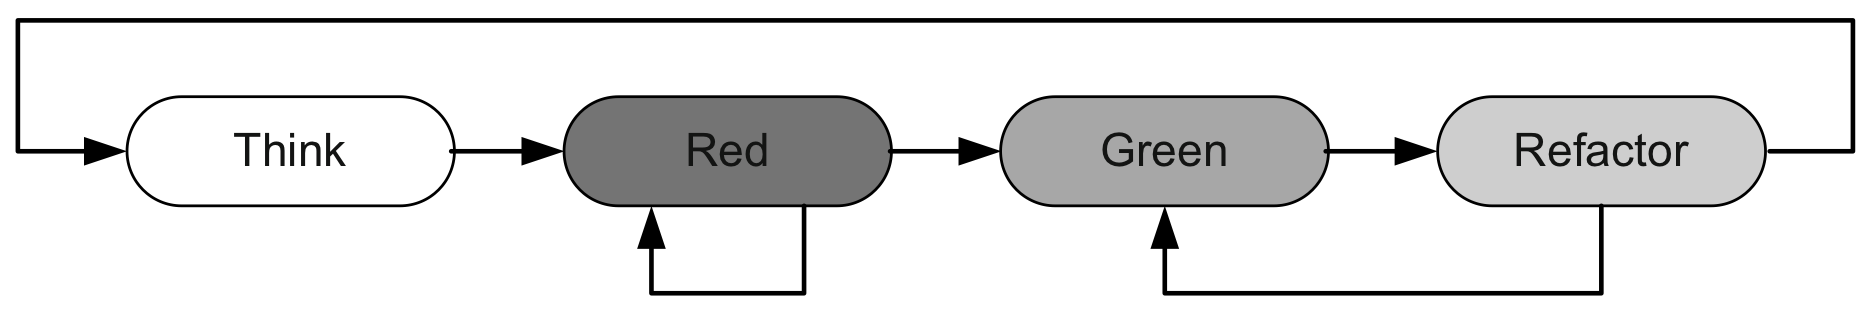
\includegraphics[clip,width=1\linewidth]{images/Phasen des TDD.png}
	\caption[Phasen des Test-Driven Development]{Phasen Ablauf des Test-Driven Development \cite[S. 153]{schatten_best_2010}}
	\label{Phasen des TDD}
\end{figure}

Die Abbildung \ref{Anwendungsbeispiel TDD} zeigt einen beispielhaften schematischen Ablaufes von TDD in der Praxis. Dabei wird veranschaulicht, dass für die ausgewählten Anforderungen geeignete Testfälle erstellt werden, um die Erfüllung der Anforderung validieren zu können. In dem Anwendungsbeispiel wird für die Anforderung A drei Testfälle benötigt. Die Testläufe, welche auf der x-Achse dargestellt werden, geben den Status der Testfälle an und wechseln von „red“ in „green“, entsprechend den jeweiligen TDD-Schritten. Dabei wird ersichtlich, dass die Anforderungen schrittweise implementiert und getestet werden. Dieses Beispiel zeigt ebenfalls auf, wie durch die schnelle Rückmeldung, durch die Tests, Seiteneffekte frühzeitig entdeckt werden können. Eine Implementierung, welche für den Testfall C2 bestimmt war, bewirkte, dass nicht nur der Test C2 weiterhin fehlschlägt, sondern auch der Testfall B2. Dieser Testfall wäre wohlmöglich bei einem traditionellen Testanfall erst sehr spät entdeckt worden und müsste aufwendig korrigiert werden. \cite[S. 154]{schatten_best_2010}

\begin{figure}[h]
	\centering
	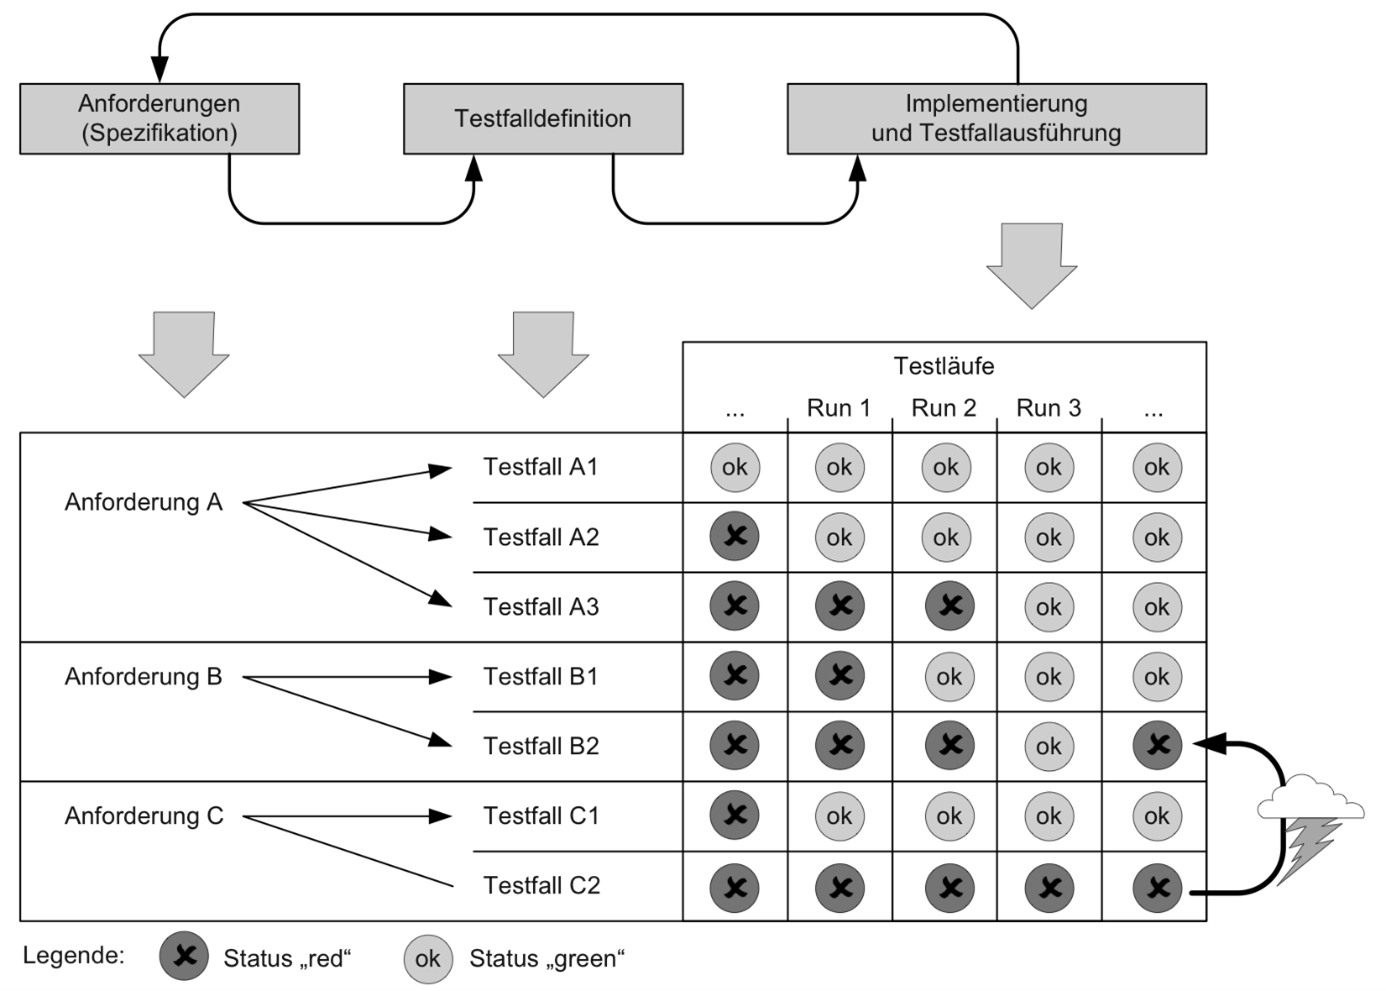
\includegraphics[clip,width=1\linewidth]{images/Anwendungsbeispiel TDD.png}
	\caption[schematischer Ablauf von Test-Driven Development in der Praxis ]{schematischer Ablauf von Test-Driven Development in der Praxis \cite[S. 154]{schatten_best_2010}}
	\label{Anwendungsbeispiel TDD}
\end{figure}


